\section{Title}

This is an R Markdown document. Markdown is a simple formatting syntax
for authoring web pages (click the \textbf{Help} toolbar button for more
details on using R Markdown).

When you click the \textbf{Knit HTML} button a web page will be
generated that includes both content as well as the output of any
embedded R code chunks within the document. You can embed an R code
chunk like this:

\begin{Shaded}
\begin{Highlighting}[]
\KeywordTok{summary}\NormalTok{(cars)}
\end{Highlighting}
\end{Shaded}

\begin{verbatim}
##      speed           dist    
##  Min.   : 4.0   Min.   :  2  
##  1st Qu.:12.0   1st Qu.: 26  
##  Median :15.0   Median : 36  
##  Mean   :15.4   Mean   : 43  
##  3rd Qu.:19.0   3rd Qu.: 56  
##  Max.   :25.0   Max.   :120
\end{verbatim}

You can also embed plots, for example:

\begin{Shaded}
\begin{Highlighting}[]
\KeywordTok{plot}\NormalTok{(cars)}
\end{Highlighting}
\end{Shaded}

\begin{figure}[htbp]
\centering
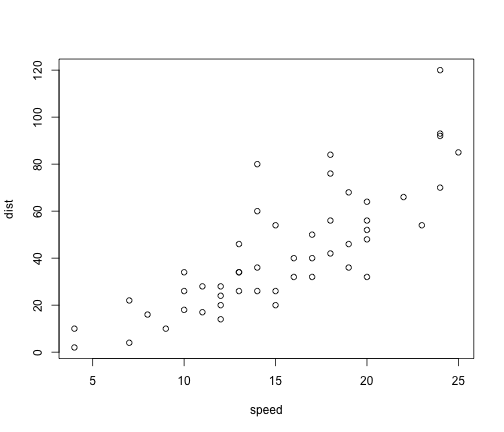
\includegraphics{figure/unnamed-chunk-2.png}
\caption{plot of chunk unnamed-chunk-2}
\end{figure}
